\documentclass{article}
\usepackage{tikz}
\usetikzlibrary{positioning}

\begin{document}

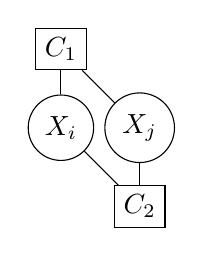
\begin{tikzpicture}[node distance=1cm]
    % Define nodes
    \node[draw, circle] (X_i) {$X_i$};
    \node[draw, circle, right of=X_i] (X_j) {$X_j$};
    \node[draw, rectangle, above of=X_i] (C_1) {$C_1$};
    \node[draw, rectangle, below of=X_j] (C_2) {$C_2$};

    % Draw edges
    \draw (X_i) -- (C_1);
    \draw (X_j) -- (C_1);
    \draw (X_i) -- (C_2);
    \draw (X_j) -- (C_2);
\end{tikzpicture}

\end{document}